\documentclass[aps,prd,11pt,tightenlines,superscriptaddress,nofootinbib,preprintnumbers,notitlepage]{revtex4-1}
 
\pdfoutput=1
\usepackage{amsmath,multirow,graphicx,tabularx,epsfig}
\usepackage{color}
\usepackage{hyperref}
 
%\newcommand{\ps}[1]{{\color{blue} [Peter] #1}}
%\newcommand{\tp}[1]{{\color{cyan} [Tilman] #1}}
%\newcommand{\fk}[1]{{\color{red} [Felix] #1}}


\def\contentsname{{\normalsize Content}}
\def\tablename{Table}
\def\figurename{Figure}

\def\pveto{P_\text{veto}}
\def\nj{n_\text{jets}}
\def\meff{m_\text{eff}}
\def\ptmin{p_T^\text{min}}
\def\gtot{\Gamma_\text{tot}}
\def\as{\alpha_s}
\def\az{\alpha_0}
\def\gz{g_0}
\def\w{\vec{w}}
\def\sdag{\Sigma^{\dag}}
\def\s{\Sigma}
\newcommand{\psib}{\overline{\psi}}
\newcommand{\Psib}{\overline{\Psi}}
%\newcommand{\dslash}{\not{\hbox{\kern-3pt $\partial$}}}
%\newcommand{\Dslash}{\not{\hbox{\kern-3pt $D$}}}
%\def\one{\leavevmode\hbox{\small1\kern-7.3pt\normalsize1}}
%%\def\one{I}
\newcommand\one{\leavevmode\hbox{\small1\normalsize\kern-.33em1}}
\newcommand{\Mpl}{M_\mathrm{Pl}}
%\def\dslash{\not{\hbox{\kern-4pt $\partial$}}}
%\def\Dslash{\not{\hbox{\kern-4pt $D$}}}
\newcommand{\p}{\partial}
\newcommand{\mat}{\mathcal{M}}
\newcommand{\lag}{\mathcal{L}}
\newcommand{\ord}{\mathcal{O}}
\newcommand{\ope}{\mathcal{O}}
\newcommand{\qqquad}{\qquad \qquad}
\newcommand{\qqqquad}{\qquad \qquad \qquad}
 
\newcommand{\ds}{\displaystyle}
\newcommand{\qb}{\bar{q}}
\newcommand{\matx}{|\mathcal{M}|^2}
%\newcommand{\mat}{\mathcal{M}}
%\newcommand{\slashed}[1]{\ensuremath{{#1}{\!}{\!}{\!}{\!}{\:}/}}
\newcommand{\really}{\stackrel{!}{=}}
\newcommand{\msbar}{\overline{\text{MS}}}
\newcommand{\qns}{f_q^\text{NS}}
\newcommand{\lqcd}{\Lambda_\text{QCD}}
\newcommand{\met}{\slashchar{p}_T}
\newcommand{\pmiss}{\slashchar{\vec{p}}_T}

\newcommand{\sq}{\tilde{q}}
\newcommand{\go}{\tilde{g}}
\newcommand{\st}[1]{\tilde{t}_{#1}}
\newcommand{\stb}[1]{\tilde{t}_{#1}^*}
\newcommand{\nz}[1]{\tilde{\chi}_{#1}^0}
\newcommand{\cp}[1]{\tilde{\chi}_{#1}^+}
\newcommand{\cm}[1]{\tilde{\chi}_{#1}^-}
\newcommand{\CP}{CP}

% all the masses 
\providecommand{\mg}{m_{\tilde{g}}}
\providecommand{\mst}[1]{m_{\tilde{t}_{#1}}}
\newcommand{\msn}[1]{m_{\tilde{\nu}_{#1}}}
\newcommand{\mch}[1]{m_{\tilde{\chi}^+_{#1}}}
\newcommand{\mne}[1]{m_{\tilde{\chi}^0_{#1}}}
\newcommand{\msb}[1]{m_{\tilde{b}_{#1}}}
\newcommand{\vsm}{\ensuremath{v_\text{SM}}}

% units of measure
\newcommand{\mev}{\text{MeV}}
\newcommand{\gev}{\text{GeV}}
\newcommand{\tev}{\text{TeV}}
\newcommand{\fb}{\text{fb}}
\newcommand{\ab}{\text{ab}}
\newcommand{\pb}{\text{pb}}
\newcommand{\br}{\text{BR}}
\newcommand{\sign}{\text{sign}}
\newcommand{\iab}{\text{ab}^{-1}}
\newcommand{\ifb}{\text{fb}^{-1}}
\newcommand{\ipb}{\text{pb}^{-1}}
\newcommand{\itevx}{\text{TeV}^{-2}}

% really great macro by Chris Lester
\def\slashchar#1{\setbox0=\hbox{$#1$}           % set a box for #1
   \dimen0=\wd0                                 % and get its size
   \setbox1=\hbox{/} \dimen1=\wd1               % get size of /
   \ifdim\dimen0>\dimen1                        % #1 is bigger
      \rlap{\hbox to \dimen0{\hfil/\hfil}}      % so center / in box
      #1                                        % and print #1
   \else                                        % / is bigger
      \rlap{\hbox to \dimen1{\hfil$#1$\hfil}}   % so center #1
      /                                         % and print /
   \fi}
\newcommand{\dslash}{\slashchar{\partial}}
\newcommand{\Dslash}{\slashchar{D}}

\newcommand{\eg}{\textsl{e.g.}\;}
\newcommand{\ie}{\textsl{i.e.}\;}
\newcommand{\Ie}{\textsl{I.e.}\;}
\newcommand{\etal}{\textsl{et al}\;}
\DeclareMathOperator{\tr}{Tr}

% maximal number of floating environments on each page 
\setlength{\floatsep}{0pt}
\setcounter{topnumber}{1}
\setcounter{bottomnumber}{1}
\setcounter{totalnumber}{1}
\renewcommand{\topfraction}{1.0}
\renewcommand{\bottomfraction}{1.0}
\renewcommand{\textfraction}{0.0}
\renewcommand{\thefootnote}{\fnsymbol{footnote}}

\newcommand{\rig}{\rightarrow}
\newcommand{\lrig}{\longrightarrow}
\renewcommand{\d}{{\mathrm{d}}}
\newcommand{\be}{\begin{eqnarray*}}
\newcommand{\ee}{\end{eqnarray*}}
\newcommand{\gl}[1]{(\ref{#1})}
\newcommand{\ta}[2]{ \frac{ {\mathrm{d}} #1 } {{\mathrm{d}} #2}}
\newcommand{\bee}{\begin{eqnarray}}
\newcommand{\eee}{\end{eqnarray}}
\newcommand{\beeq}{\begin{equation}}
\newcommand{\eeeq}{\end{equation}}
\newcommand{\mc}{\mathcal}
\newcommand{\mr}{\mathrm}
\newcommand{\ep}{\varepsilon}
\newcommand{\eps}{\varepsilon}
%\renewcommand{\vec}{\bf}
\newcommand{\emt}{$\times 10^{-3}$}
\newcommand{\emfo}{$\times 10^{-4}$}
\newcommand{\emfi}{$\times 10^{-5}$}

\newcommand{\revision}[1]{{\bf{}#1}}

\newcommand{\hzero}{h^0}
\newcommand{\Hzero}{H^0}
\newcommand{\Azero}{A^0}
\newcommand{\PHiggs}{H}
\newcommand{\PW}{W}
\newcommand{\PZ}{Z}

\newcommand{\sw}{\ensuremath{s_w}}
\newcommand{\cw}{\ensuremath{c_w}}
\newcommand{\swd}{\ensuremath{s^2_w}}
\newcommand{\cwd}{\ensuremath{c^2_w}}
%
%% 2HDM Higgs masses
\newcommand{\mhhd}{\ensuremath{m^2_{\Hzero}}}
\newcommand{\mhh}{\ensuremath{m_{\Hzero}}}
\newcommand{\mlhd}{\ensuremath{m^2_{\hzero}}}
\newcommand{\Mlh}{\ensuremath{m_{\hzero}}}
\newcommand{\mad}{\ensuremath{m^2_{\Azero}}}
% \newcommand{\ma}{\ensuremath{m_{\Azero}}}
\newcommand{\mhpd}{\ensuremath{m^2_{\PHiggs^{\pm}}}}
\newcommand{\mhp}{\ensuremath{m_{\PHiggs^{\pm}}}}

%% GPS: the following defs have been commented out
%%      because one of them interfered with the \url package
%\newcommand{\sa}{\ensuremath{\sin\alpha}}
%\newcommand{\ca}{\ensuremath{\cos\alpha}}
%\newcommand{\cad}{\ensuremath{\cos^2\alpha}}
%\newcommand{\sad}{\ensuremath{\sin^2\alpha}}
%\newcommand{\sbd}{\ensuremath{\sin^2\beta}}
%\newcommand{\cbd}{\ensuremath{\cos^2\beta}}
%\newcommand{\cb}{\ensuremath{\cos\beta}}
%\renewcommand{\sb}{\ensuremath{\sin\beta}}
%\newcommand{\tanbd}{\ensuremath{\tan^2\beta}}
%\newcommand{\cotbd}{\ensuremath{\cot^2\beta}}
%\newcommand{\tanb}{\ensuremath{\tan\beta}}
%\newcommand{\tb}{\ensuremath{\tan\beta}}
%\newcommand{\cotb}{\ensuremath{\cot\beta}}


% trying to make it look okay for A4 and for letter formats
%\addtolength{\topmargin}{10mm}
\addtolength{\evensidemargin}{-5mm}
\addtolength{\oddsidemargin}{-5mm}
%\addtolength{\textheight}{5mm}
\addtolength{\textwidth}{10mm}

\newcommand{\hepstore}{\texttt{HepStore}}
\newcommand{\python}{\texttt{Python~2.7}}

\usepackage{framed}
\usepackage{listings}
\usepackage{color}

\definecolor{dkgreen}{rgb}{0,0.6,0}
\definecolor{gray}{rgb}{0.5,0.5,0.5}
\definecolor{mauve}{rgb}{0.58,0,0.82}

\lstset{frame=tb,
  language=Python,
  aboveskip=3mm,
  belowskip=3mm,
  showstringspaces=false,
  columns=flexible,
  basicstyle={\small\ttfamily},
  numbers=none,
  numberstyle=\tiny\color{gray},
  keywordstyle=\color{blue},
  commentstyle=\color{dkgreen},
  stringstyle=\color{mauve},
  breaklines=true,
  breakatwhitespace=true,
  tabsize=3
}

%%%%%%%%%%%%%%%%%%%%%%%%%%%%%%%%%%%%%%%%%%%%%%%%%%%%%%%%%%%%%%%%%%%%%%%%
\begin{document}
 
\title{{\bf\Huge\hepstore: The Awakening}}

\preprint{IPPP/16/72}

\author{Peter Schichtel}
\affiliation{Institute for Particle Physics Phenomenology, Durham University, UK}
\email{peter.schichtel@durham.ac.uk}


\begin{abstract}
  A framework to trade (hence the name) your phenomelogy analysis in a preserved way. 
\end{abstract}

\maketitle

\bigskip 
\bigskip 

\tableofcontents 

\newpage

%%%%%%%%%%%%%%%%%%%%%%%%%%%%%%%%%%%%%%%%%%%%%%%%%%%%%%%%%%%%%%%%%%%%%%%%

\section{Installation}
\label{sec:installation}

The \hepstore~--~Framework is written solely in \python. To install the package you need 'pip'~\cite{}.
%
\begin{framed}
  \begin{center}
    pip install (-{}-upgrade) (-{}-user) git+https://github.com/PeterSchichtel/hepstore.git
  \end{center}
\end{framed}
%
The arguments in parenthesis are optional. Furthermore, if you want to make use of the {\bf Monte~Carlo reproducability features} in \hepstore~you need a working Docker~\cite{} installation.

\section{The \hepstore~--~Framework}
\label{sec:framework}

In the following we will outly the modules hepstore is composed of. We will introduce their usage and motivation.

\subsection{hepstore.docker}

There has been tremondous effort in the experimantal community to achieve high scientific standards of reproducibility. Namely the ReCast and Reana frame works. However, one should not think that no such efforts have been undertaken in the phenomelogical community. There is MadAnalysis5 which has the ability to recast LHC analyses. There is, of course, Rivet, which comes along with verified phenomenolgical and experimental analyses. These tools provide building blocks to perform, save and redo an analysis. In addition the MC community develops ever simpler installation routines for their code packages, including interfaces to third party software. So, why bother with recasting respectively reproducing phenomenoligical results? Anybody who has ever tried to redo what they did five years ago might already know the answer: library missing, code missing, data missing, does not compile anymore, does not run anymore, 32-bit what?, not supported, what was the random seed again, which version of package X was used, etc. pp. So part of this work will be to show a recipe to solve this problem (once and for all, hopefully).

The short answer is Docker. For those who know Docker and are ready to critisize this solution and those who do not know Docker a more lengthy argument follows. Docker is a program which allows to containerize applications. This means once a Docker container is produced, the whole state of the system is fixed. This imidiately clears all of the points raised above. One cannot loose code or a library anymore. It's all in the docker image. The docker image itself can be stored locally, of course, as well as on the docker webpage. There it can be made accessible. This means anybody can reproduce your analysis in the exact state it was developed and used. However, this work wants to be more than just an advertisement for Docker. There is an other issue with MC production and analysis, which has to be considered for proper reproducibility. That is the steering and interaction of the analysis steps. This is what hepstore.docker provides. First there is an easy to use interface to any docker image, which can be used from within \python.
%
\begin{lstlisting}
# module: hepstore.docker.interface

# imports for this module
import docker
import os

# the actual interface class
class DockerIF(object):

    # cosntructor
    def __init__( self,
                  image="GENERATOR",
                  version="TAG",
                  verbose=False ):
        # save arguments
        self.IMAGE   = image
        self.TAG     = version
        self.name    = "%s:%s" % (self.IMAGE,self.TAG)
        self.verbose = verbose
        # connect to docker
        self.client  = docker.from_env()
        # check if docker image exist otherwise try to pull
        if not len(self.client.images.list(name=self.IMAGE))>0:
            print "--%s: pull image" % self.name
            self.client.images.pull(self.IMAGE,tag=self.TAG)
            pass
        pass

    # actual command run interface
    def run(self,args,directory=None,verbose=False):
        # construct docker container name
        containername = "%s:%s" % (self.IMAGE,self.TAG)
        # see if there is a directory to be mounted from host machine
        try:
            folder    = os.path.realpath(directory)
            volume    = {folder: {'bind': '/UserVolume', 'mode': 'rw'}}
            pass
        except Exception:
            volume    = {}
            pass
        # run the command on the container
        container = self.client.containers.run( containername,
                                                command=args,
                                                volumes=volume,
                                                working_dir='/UserVolume',
                                                detach=True )
        # print the container output on screen
        for i,line in enumerate(container.logs( stdout=True, stderr=True, stream=True)):
            if self.verbose:
                print "%i: %s" % (i,line.strip())
                pass
            pass
        # remove container
        container.remove()
        pass

    pass # DockerIF
\end{lstlisting}
%

\subsubsection{Example}

As an example, we construct our own Herwig 7 interface the code can be found in App.~... This code can be called with 'hepstore-herwig' and will behave identical to the 'Herwig' command once Herwig7 would be installed on your machine. Let's say that for any reason you need another version of Herwig. As you can see from the code fragment the docker image and the docker file can be found on the docker webpage under user 'peterschichtel/herwig:7.0.4'. you can use the dockerfile found there and generate your own version of Herwig, say 'yourname/herwig:7.1.0', by altering it correspondingly .Now you can produce MC events with the interface given here: 'hepstore-herwig --repository yourname --generator-version 7.1.0 build yourRunCard.in'. So far so good. Now you'd like to use the 'rivet-mkhtml' command to plot these things you computed. However, there is no special hepstore-rivet-mkhtml you could use. Note that rivet here is a pseudonyme for any command that is not included in the hepstore.docker family which you might need. In this sepcific case the solution is very simple. Copy the above code into a new file rivet-mkhtml.py. In the last command change 'Herwig' to 'rivet-mkhtml' (this is possible because the herwig installation comes along with a rivet installation). use chmod to make the python file executable and just run './rivet-mkhtml.py --repository yourname --generator-version 7.1.0 yourListOfRivetCommandsAndFilePathes' as usual, done. If you think that this is just a more complicated way of running your analysis, don't be mistaken. Something happend on the way: you produced a dockerfile as well as a docker image. This preserves your whole internal state of your code and analysis! Your full analysis has become reproducible for the future by providing two files as supplimential material in your publication: your self written 'rivet-mkhtml' interface and the dockerfile. Even better, if you are up to it you can contribute to hepstore by adding your rivet interface to the hepstore.docker family and upload your docker image to the docker webpage. Your complete production and analysis state is now preserved and interfaced for future use, by publishing the your herwig run card and the following bash snippet:
%
\begin{lstlisting}[language=Bash]
  #!/usr/bin/env bash
  pip install git+https://github.com/PeterSchichtel/hepstore.git
  hepstore-herwig --repository yourname --generator-version 7.1.0 read yourRunCard.in
  hepstore-herwig --repository yourname --generator-version 7.1.0 run  yourRunCard.run
  hepstore-rivet-mkhtml --repository yourname --generator-version 7.1.0 yourListOfRivetCommandsAndFilePathes
\end{lstlisting}
%
This example is where \hepstore~ takes its name from. You can add and publish your own product for other's to be used when they want to build on or reproduce your research. Furthermore, it i sthe authors hope that the community might provide official docker images to be used as well.

\subsection{hepstore.plot}

In the case where you are not able to use the rivet or madanalysis plotting capabilities, \hepstore provides a simple user interface 'hepstore-plot' which can plot any one or two dimensional representation of your data\footnote{provided in .npy format}. Currently the following kinds of plots are suported: scatter, histogram, errorbar, line, errorband, and contour.

\subsubsection{Data Format}

\hepstore~uses the '.npy' format

\subsubsection{Example}
produce some data
%
\begin{lstlisting}
#!/usr/bin/env python

# module examples/hepstore_plot produce_data

# import for this module
import numpy as np

# number of events
nevents = 20000

# generate data set I
mean = np.array([0.0,0.0])
cov  = np.array([[1.0,0.0],[0.0,1.0]])
data = np.random.multivariate_normal(mean, cov, 2*nevents)
np.save('data_1.npy',data)

# generate data set II
mean = np.array([2.5,-2.5])
cov  = np.array([[1.0,0.0],[0.0,1.0]])
data = np.random.multivariate_normal(mean, cov, nevents)
mean = np.array([-1.4,0.8])
cov  = np.array([[0.02,1.2],[-1.7,0.01]])
data = np.concatenate((data,np.random.multivariate_normal(mean, cov, nevents)))
np.save('data_2.npy',data)

\end{lstlisting}
%
plot with hepstore-plot
%
\begin{lstlisting}[language=Bash]
#!/usr/bin/env bash

## produce data for this example
./produce_data.py

## plot scatter
hepstore-plot -f data_1.npy data_2.npy -k scatter \
	      -c blue red \
	      --xmin -5 --xmax 5 \
	      --ymin -5 --ymax 5 \
	      --legend 'single gaussian' 'double gaussian' \
	      --alpha 0.6 \
              --title 'example plot a.)' 'scatter'\
	      --path $(pwd)/example_a.pdf

## plot histogram of x axis
hepstore-plot -f data_1.npy data_2.npy -k histogram \
	      -a 0 \
	      -c blue red \
	      --normed \
	      --bins 20 \
	      --xmin -5 --xmax 5 \
	      --ymax 0.6 \
	      --ylabel '$\rho(x)$' \
	      --legend 'single gaussian' 'double gaussian' \
	      --alpha 0.6 \
	      --title 'example plot b.)' 'histogram'\
	      --path $(pwd)/example_b.pdf

## plot histogram of x axis
hepstore-plot -f data_1.npy data_2.npy -k histogram \
	      -a 1 \
	      -c blue red \
	      --normed \
	      --bins 20 \
	      --xmin -5 --xmax 5 \
	      --ymax 0.6 \
	      --xlabel 'y' \
	      --ylabel '$\rho(y)$' \
	      --legend 'single gaussian' 'double gaussian' \
	      --alpha 0.6 \
	      --title 'example plot c.)' 'histogram'\
	      --path $(pwd)/example_c.pdf
\end{lstlisting}
%
show plots
%
\begin{figure}
  \centering
  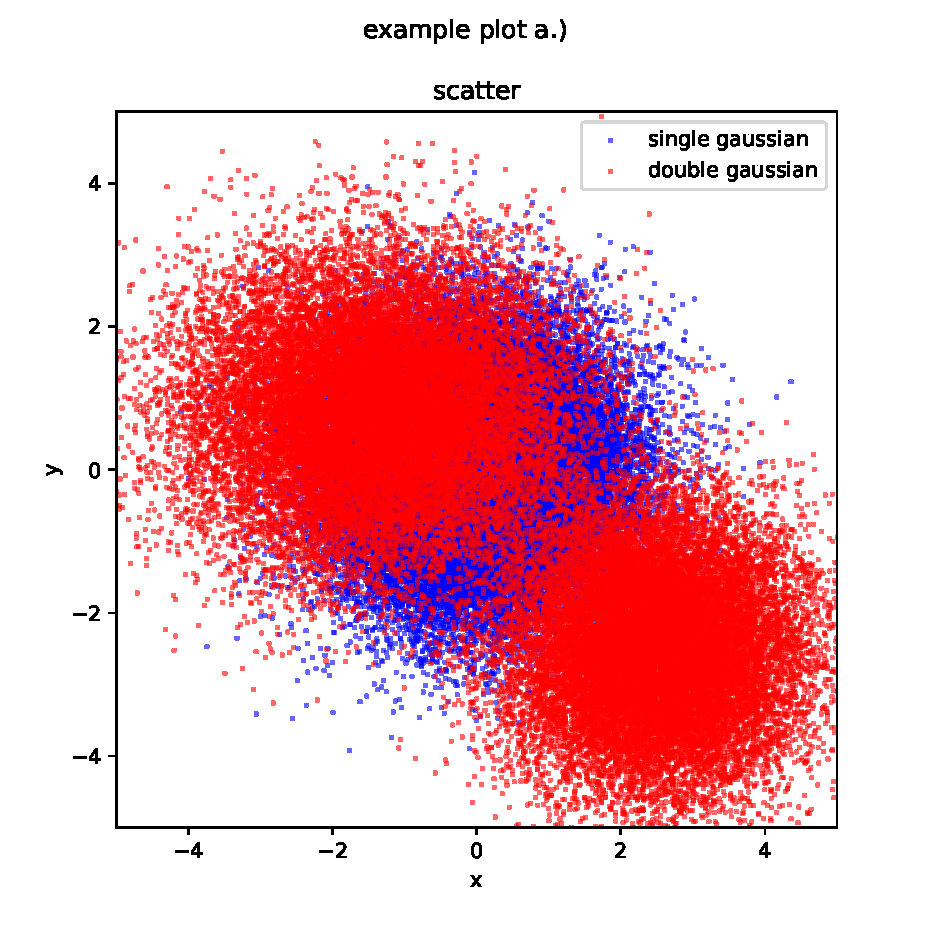
\includegraphics[width=0.3\textwidth]{../examples/hepstore_plot/example_a.pdf}
  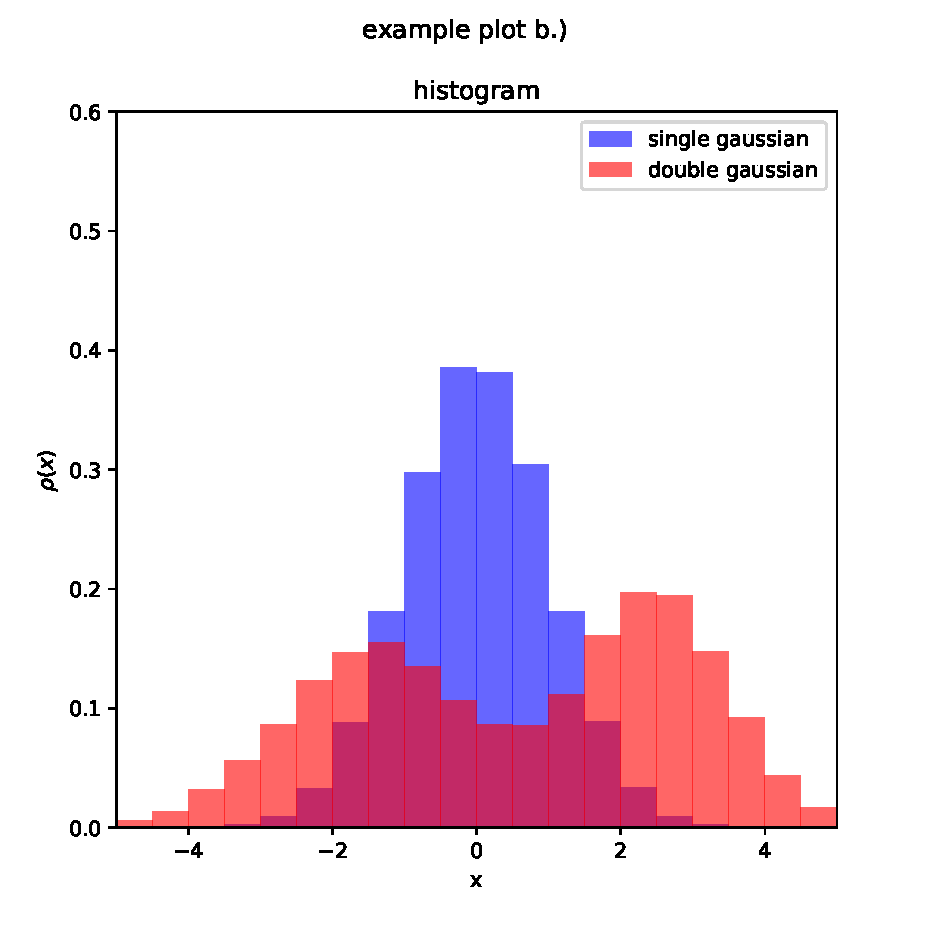
\includegraphics[width=0.3\textwidth]{../examples/hepstore_plot/example_b.pdf}
  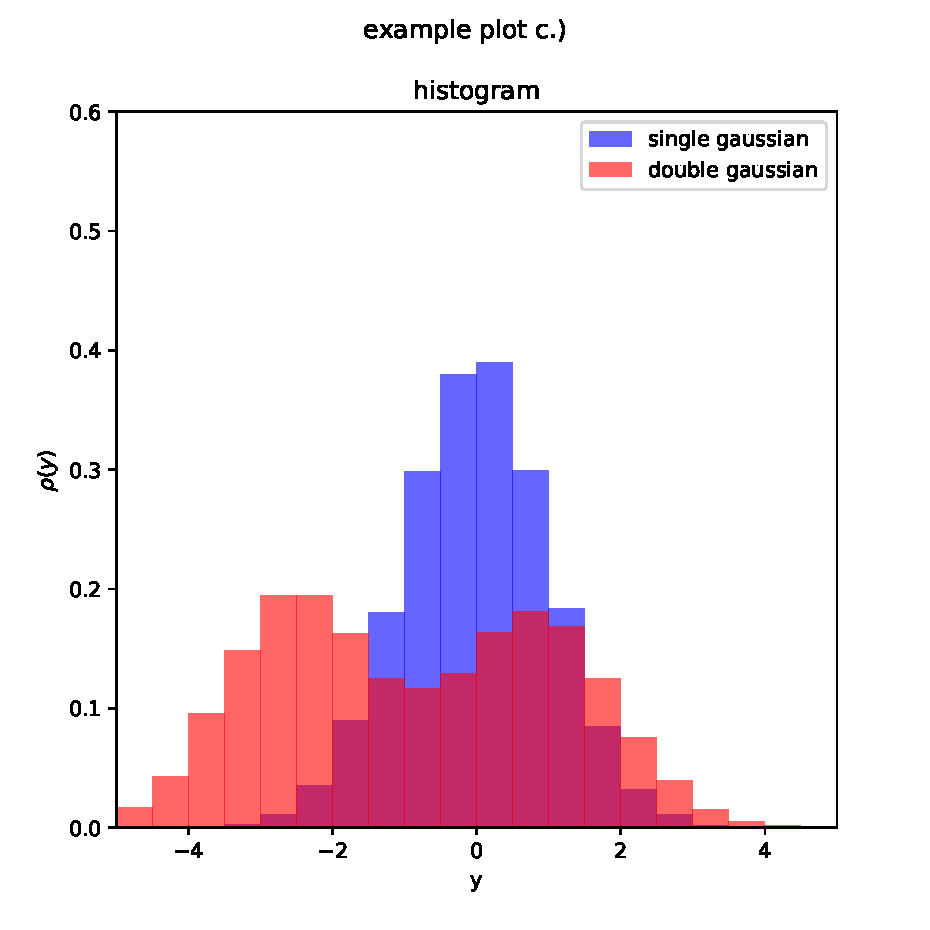
\includegraphics[width=0.3\textwidth]{../examples/hepstore_plot/example_c.pdf}
  \caption{}
  \label{fig:example_plotting}
\end{figure}
%


\subsection{hepstore.school}

One of the themes very interesting to particle physiscts and also recieving more and more attention in the phenomenolgical community is machine learning. 'hepstore.school' is an attempt to provide a genric interface to python's sklearn package. our school consists of a teacher, a student and, of course, a book. the teacher advices the student which algorithm to use, where upon the student takes the algorithm from the book and is able to explore and train itself to learn from the data provided.

\subsubsection{Classifiers}

lda,qcd,svc,mlp

\subsubsection{Tuning}

As it is not a prior clear which parameters to chose for an algorithm, 'hepstore-school' provides the switch '-{}-only\_explore' which will try to automatically find the best parameters for the given training set. In addition for all numerical parameters it provides cross validation plots to check for over respectively under performance. Note that some classifiers might have a large parameter space and hence can not be tunde in a fully automated way, yet.

\subsubsection{Training}

Training is performed automattically on a $75\%$ subset of the data provided.

\subsubsection{Testing}

Training is performed automattically on a $25\%$ subset of the data provided.

\subsubsection{Example}

same data as above

%
\begin{lstlisting}[language=Bash]
  #!/usr/bin/env bash

## produce data for this example
./produce_data.py

## tune quadratic linear discriminant
hepstore-school -c qda -f $(pwd)/data_1.npy $(pwd)/data_2.npy \
		-l 0.0 1.0 --only_explore \
		--random_state 7 \
		--path $(pwd)/tuning

## which yields:--QDA: explore
#--info: RandomizedSearchCV took 24.36 seconds for 200 candidates parameter settings.
#--info: Model with rank: 1
#--info: Mean validation score:  8.06e-01 (std:  3.28e-03)
#--info: Parameters: {'reg_param': 0.0027454802945078294, 'tol': 0.00072971227653656045}
#--info: Model with rank: 2
#--info: Mean validation score:  8.05e-01 (std:  3.19e-03)
#--info: Parameters: {'reg_param': 0.00862957001583331, 'tol': 0.00068120836729054681}
#--info: Model with rank: 3
#--info: Mean validation score:  8.05e-01 (std:  3.19e-03)
#--info: Parameters: {'reg_param': 0.014999438477383165, 'tol': 0.00091459513377715248}

## plot cross validation
vars=('reg_param' 'tol')
for var in ${vars[@]} ; do
    hepstore-plot -f $(pwd)/tuning/train_scores_${var}.npy \
		  $(pwd)/tuning/test_scores_${var}.npy \
		  -k errorband --logx \
		  --legend 'train' 'test' \
		  -c yellow blue \
		  --title "Cross validation QDA" \
		  --xlabel "$var" \
		  --ylabel 'score' \
		  --path $(pwd)/$var.pdf
done

## perform the actuall machine learning
hepstore-school -c qda -f $(pwd)/data_1.npy $(pwd)?data_2.npy \
		-l 0.0 1.0 \
		--reg_param 0.002745 --tol 0.0007291 \
		--random_state 7 \
		--path $(pwd)/learning

## ROC curve
hepstore-plot -f $(pwd)/learning/roc.npy -k line \
	      --legend 'ROC' \
	      -c black \
	      --title "ROC curve QCD" \
	      --xlabel '$\epsilon_{S}$' \
	      --ylabel '$1-\epsilon_{B}$' \
	      --path $(pwd)/roc.pdf

## probability map
hepstore-plot -f $(pwd)/data_1.npy $(pwd)/data_2.npy \
	      $(pwd)/learning/probability_map.npy \
	      -k "2*scatter" contour \
	      -c blue red Blues \
	      --xmin -5 --ymin -5 --xmax 5 --ymax 5 \
	      --alpha 0.3 \
	      --legend 'background' 'signal' \
	      --title "probability map QDA" \
	      --path $(pwd)/probbility_map.pdf
\end{lstlisting}
%
show plots
%
\begin{figure}
  \centering
  \includegraphics[width=0.22\textwidth]{../examples/hepstore_school/tol.pdf}
  \includegraphics[width=0.22\textwidth]{../examples/hepstore_school/reg_param.pdf}
  \includegraphics[width=0.22\textwidth]{../examples/hepstore_school/roc.pdf}
  \includegraphics[width=0.22\textwidth]{../examples/hepstore_school/probability_map.pdf}
  \caption{}
  \label{fig:example_plotting}
\end{figure}
%


\subsection{hepstore.analysis}

the hepstore-analysis module is a high level package to perform the usual statistical computations needed in high energy physics. it utilizes hepstore.school to provide signal and background classification and extract statistical quantities such as the maximal poissonian significance, the upper exclusion bound on the signal cross section etc.

still missing: traditional cut analysis

\subsubsection{Example}

\section{hepstore-eas: produce and anlyse Extended Air Showers the \hepstore~way}

\subsection{List}
'hepstore-eas -L'

As this is a specific air shower framework we organise everything with respect to the following scheme: energy -> primary particle -> physical process -> MC generator -> nucleon model -> final state
the -{}-list argument searches for this structure and lists the following possible contents
hard events -> attempted showers -> showeres -> observables

\subsection{Generation}

'hepstore-eas -G'

we interface from the hepstore.docker family (more details in appendix) and provide automated runcards for herwig to produce events which may be showerd by corsika

\subsubsection{Nucleon Modle}

we provide two nucleon models 'full' and 'fragmented'

\subsection{Shower}

'hepstore-eas -S'

we interface from the hepstore.docker family and provide automated runcards for corsika to either shower events generted with '-G' or produce corsika stand alone showers (internal corsika di-jet production) when using '-C 7.4' (here 7.4 is the version vor the docker image)

\subsection{Observables}

'hepstore-eas -A'

we provide our own event class to read corsika produced extended air showers. inspired by rivet we allow for dynamic load of user analysis modules and provide one example for such, constructing $\rho_\mu$ and $X_\text{max}$. hepstore-eas automatically provides its output in .npy format

\subsection{Example}

\subsubsection{A User Analysis}

\subsubsection{Comparing Herwig 7 di-jet production with internal Corsika QCD model}

\section{Contributions and Requests}

\section{Conclusions}

\begin{appendix}

  \section{The hepstore.docker family}

  \subsection{hepstore-herwig}

  \subsubsection{Code}

  %
  \begin{lstlisting}
# module: hepstore.docker.herwig

# imports for this module
import os

############################################################################
## run the app
############################################################################
def main(args=None):

    # we need to setup the arg parser
    import argparse
    parser = argparse.ArgumentParser(
        description =
        "This App allows to run the Herwig code out of the box with python 2.7." )
    
    # specify arguments for versioning
    parser.add_argument( "--repository"       ,
                         type    = str,
                         default = "peterschichtel",
                         help    = "docker repo of the genrator" )
    parser.add_argument( "--generator"        ,
                         type    = str,
                         default = "Herwig",
                         help    = "which generator to run, default Herwig " )
    parser.add_argument( "--generator-version",
                         type    = str,
                         default = "7.0.4",
                         help    = "which version to run, default 7.0.4" )
    
    # mount a directory
    parser.add_argument( "--directory",
                         type    = str,
                         default = os.getcwd(),
                         help    =
                         "mount this directoy as /UserDirectory (automatic working dir!), default is PWD!" )

    # verbose stdout
    parser.add_argument( "-v", "--verbose",
                         action  = "store_true",
                         help    = "print container stdout" )
    
    # parse args
    parsed_args, unknown = parser.parse_known_args(args)
            
    # run the app
    from interface import DockerIF as Herwig
    app=Herwig(
        image     = os.path.join( parsed_args.repository.lower(),
                                parsed_args.generator.lower() ),
        version   = parsed_args.generator_version,
        verbose   = parsed_args.verbose
    )
    app.run(
        directory = parsed_args.directory,
        args       = [ '/bin/bash',
                       '-c',
                       'source $ACTIVATE && %s ' % " ".join(['Herwig'] + unknown )
        ]
    )
        
    pass # main
############################################################################

############################################################################
if __name__ == "__main__":
    main()
    pass
############################################################################
  \end{lstlisting}
  %

  \subsubsection{Dockerfile}
  
  \subsection{hepstore-corsika}

  \subsubsection{Code}

  \subsubsection{Dockerfile}
  
  \subsection{hepstore-hepmc2corsika}

  \subsubsection{Code}

  \subsubsection{Dockerfile}

\end{appendix}


\end{document}
 
 
 

 
 




